\documentclass[10pt]{beamer}

\usetheme[
%%% options passed to the outer theme
%    hidetitle,           % hide the (short) title in the sidebar
%    hideauthor,          % hide the (short) author in the sidebar
%    hideinstitute,       % hide the (short) institute in the bottom of the sidebar
%    shownavsym,          % show the navigation symbols
%    width=2cm,           % width of the sidebar (default is 2 cm)
%    hideothersubsections,% hide all subsections but the subsections in the current section
%    hideallsubsections,  % hide all subsections
    left               % right of left position of sidebar (default is right)
%%% options passed to the color theme
%    lightheaderbg,       % use a light header background
  ]{AAUsidebar}

% If you want to change the colors of the various elements in the theme, edit and uncomment the following lines
% Change the bar and sidebar colors:
%\setbeamercolor{AAUsidebar}{fg=red!20,bg=red}
%\setbeamercolor{sidebar}{bg=red!20}
% Change the color of the structural elements:
%\setbeamercolor{structure}{fg=red}
% Change the frame title text color:
%\setbeamercolor{frametitle}{fg=blue}
% Change the normal text color background:
%\setbeamercolor{normal text}{bg=gray!10}
% ... and you can of course change a lot more - see the beamer user manual.


\usepackage[latin1]{inputenc}
\usepackage{comment}
\usepackage{lmodern}
\usepackage{ucs}
\usepackage{t1enc}
\usepackage[english]{babel}
\usepackage[T1]{fontenc}
% Or whatever. Note that the encoding and the font should match. If T1
% does not look nice, try deleting the line with the fontenc.
\usepackage{helvet}

\usepackage{subcaption}
\captionsetup{compatibility=false}

% colored hyperlinks
\newcommand{\chref}[2]{%
  \href{#1}{{\usebeamercolor[bg]{AAUsidebar}#2}}%
}


\date{\today}


	\title{sw707e14 - Bicycles and the Internet of Things}
	\author[sw707e14]{Dennis Jakobsen \\
	Erik Sidelmann Jensen \\
	Lasse Vang Gravesen \\
	Lars Andersen \\
	Mathias Winde Pedersen \\
	S\o ren Skibsted Als}
	
% - Give the names in the same order as they appear in the paper.
% - Use the \inst{?} command only if the authors have different
%   affiliation. See the beamer manual for an example




% specify a logo on the titlepage (you can specify additional logos an include them in 
% institute command below
\pgfdeclareimage[height=1.5cm]{titlepagelogo}{AAUgraphics/aau_logo_new} % placed on the title page
%\pgfdeclareimage[height=1.5cm]{titlepagelogo2}{graphics/aau_logo_new} % placed on the title page
\titlegraphic{% is placed on the bottom of the title page
  \pgfuseimage{titlepagelogo}
%  \hspace{1cm}\pgfuseimage{titlepagelogo2}
}

\graphicspath{ {Media/} }
\newcommand{\btVFill}{\vskip0pt plus 1filll}

\begin{document}
% the titlepage
{\aauwavesbg%
\begin{frame}[plain,noframenumbering] % the plain option removes the sidebar and header from the title page
  \titlepage
\end{frame}}
		
	\section{Introduction}
\begin{frame}
	\begin{center}
		\Huge Introduction
	\end{center}
\end{frame}

\begin{frame}
\frametitle{Who Are We?}
\begin{itemize}
	\item Erik
	\item Lasse
	\item S�ren
	\item Lars
	\item Dennis
	\item Mathias
\end{itemize}
\end{frame}

\begin{frame}
\frametitle{What Will be in This Presentation?}
\begin{itemize}
	\item What are we dealing with? - Erik
	\item What problems are there to address? And what solutions did we consider? - Erik
	\item What is the Internet of Things and how does the solution fit within the context of that? - Lasse
	\item Technologies - Lasse
	\item How did we structure the solution? - S�ren
	\item A demonstration of the outcome. - Lars, Dennis
	\item What can be concluded from our work? - Mathias
\end{itemize}
\end{frame}

\section{Bicycle Sharing System}
\begin{frame}
	\begin{center}
		\Huge Bicycle Sharing System
	\end{center}
\end{frame}

\begin{frame}
\frametitle{What Is a Bicycle Sharing System?}
	\begin{center}
		\textit{"Short term bicycle rental available at unattended stations"} - Paul DeMaio, MetroBike LCC
	\end{center}
	
	The idea is that: "bikes provide a new paradigm in short distance transport that is a realistic alternative to the bus, tram, taxi, or private car [...]".
	\newline\newline
	Pick your bicycle at A and place it at B.
	\bigskip
	\btVFill
	\tiny source of definition: http://www.bicyclesharingsystems.com/whatis.php
\end{frame}

\begin{frame}
\frametitle{The Current System}
	%picture if there is room for it
	\begin{itemize}
		\item CIVITAS ARCHIMEDES.
		\item 2009: 135 bicycles and 19 stations.
		\item Today: +2 stations and +102 bicycles.
		\item Open system, free to use.
		\item Each bicycles is used minimum 1.4 times during a day.
		\item AFA JCDecaux.
	\end{itemize}
\end{frame}

\begin{frame}
\frametitle{Problems With the Current System}
	\begin{itemize}
		\item You do not know beforehand if there are bicycles available for you and how many.
		\item You cannot make sure that there will be a bicycle for you.
		\item There is no way for Aalborg Kommune to monitor the use of the bicycles.
	\end{itemize}
\end{frame}

\begin{frame}
\frametitle{How Can We Solve These Problems?}
	\begin{large}
	Does other bicycle sharing systems address these problems?
	\end{large}
	\begin{itemize}
		\item Status: All of the examined systems provides a website for getting the current amount of bicycles at each station.
		\item Booking: Of the examined systems it is done either by creating a special subscription, paying by week, month or quarter, or by
		creating a booking for a bicycle online in advance asking for a confirmation half an hour before reservation.
		\item Monitoring: Of the examined systems it is either done through registering bicycles in docks at the stations or by 
		tracking their position with GPS.
	\end{itemize}
\end{frame}

\section{Our Goal For the Project}

\begin{frame}
	\begin{center}
		\Huge Our Goal For the Project
	\end{center}
\end{frame}

\begin{frame}
\frametitle{Problem Definition}
	%We define the problem definition of enhancing the user experience by targeting some of the mentioned problems by this hypothesis:
	\begin{center}
		\textbf{It is possible to develop a system for Aalborg Bycykel that is user friendly and manageable, within the context of the Internet of Things.}
	\end{center}
	\begin{itemize}
		\item What are the requirements for a city bicycle booking and positioning system?
		\item How can the booking and positioning system be designed and implemented within the context of the Internet of Things?
		\item Why should the developed system be used over the currently used system?
	\end{itemize}
\end{frame}

\begin{frame}
\frametitle{Requirements}
	We want a system that is able to:
	\begin{itemize}
		\item Provide status of availability of bicycles.
		\item Give an option to book a bicycle.
		\item Track the position of each bicycle.
		\item Collect data for analysis of the usage for Aalborg Kommune.
		\item Predicting when a bicycle will be available for use.
	\end{itemize}
\end{frame}

\begin{frame}
\frametitle{Criteria}
	What values did we want the system to have?
	\begin{itemize}
		\item As little change as possible, rather an extension to the current system.
		\item Easy to use and accessible by everyone.
	\end{itemize}
\end{frame}

%Visualise the different suggestions to problems(may be too specific)
\section{Chosen Solutions}
\begin{frame}
	\begin{center}
		\Huge Chosen Solutions
	\end{center}
\end{frame}

\begin{comment}


\begin{frame}
\frametitle{Availability of Bicycles - Camera}
\begin{figure}
\centering
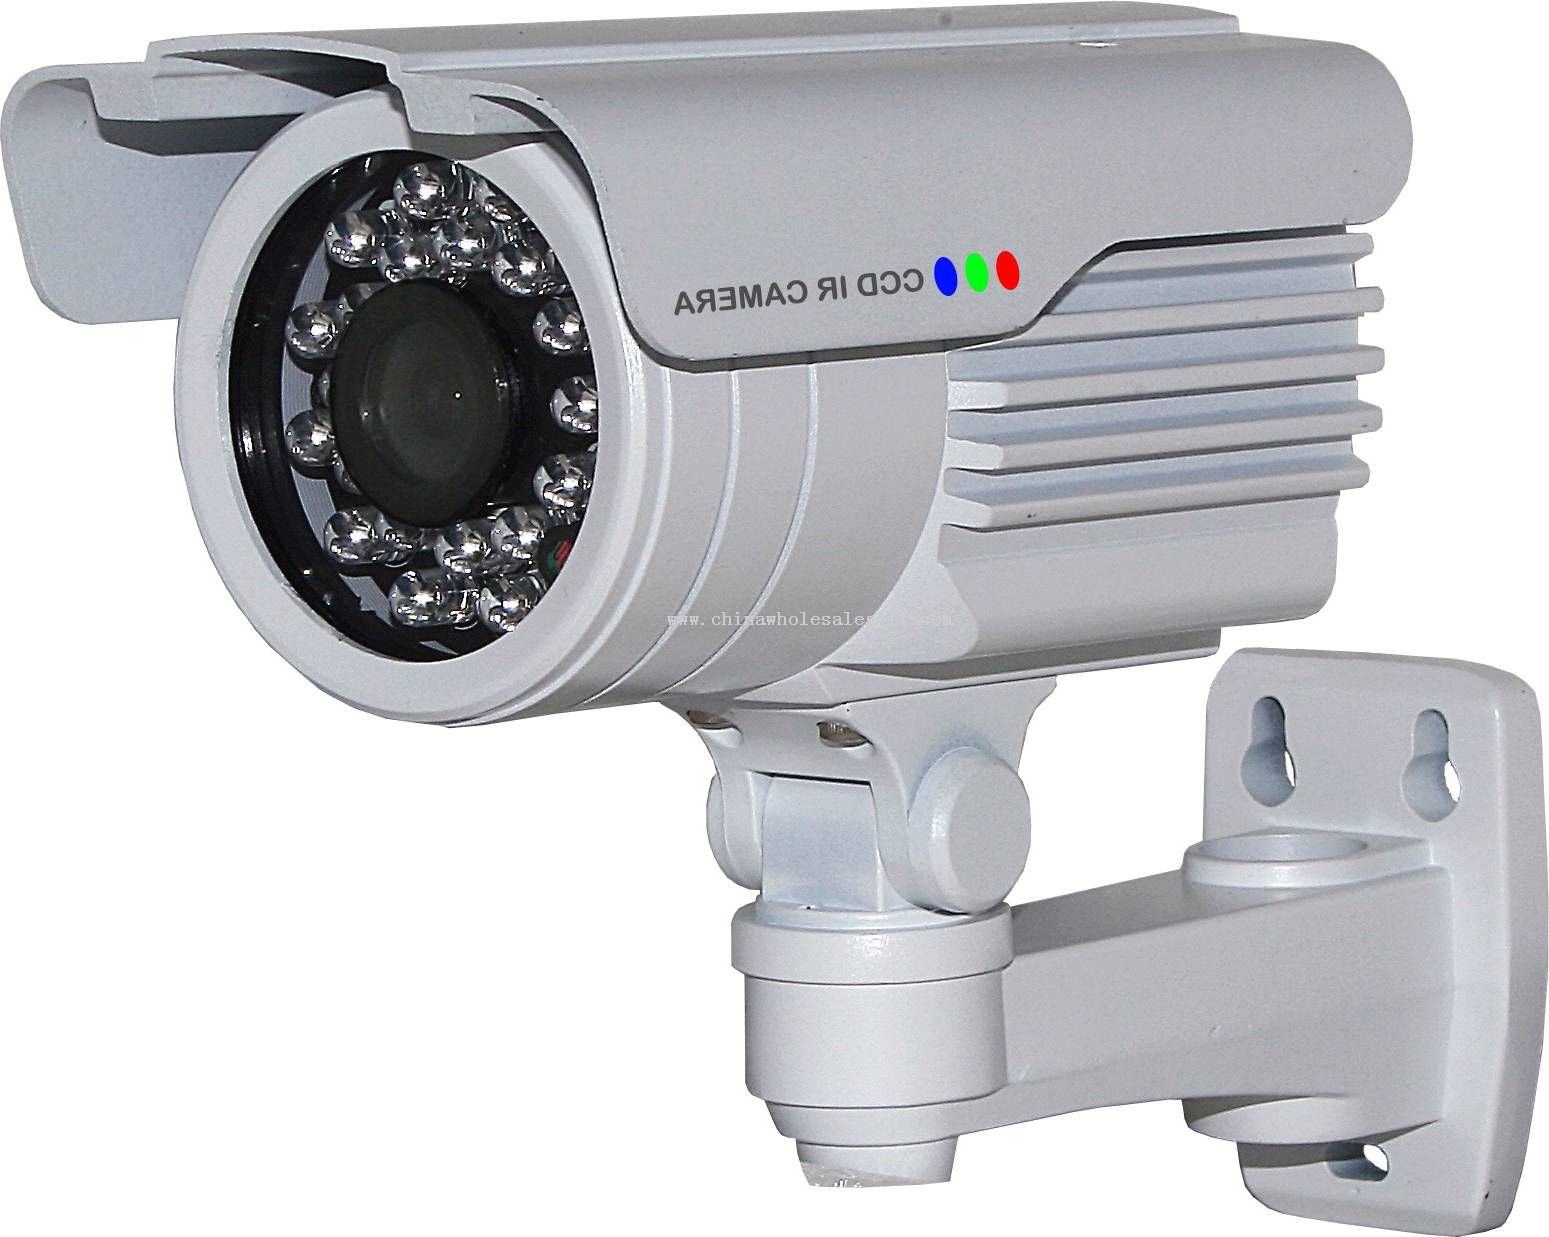
\includegraphics[scale=0.05]{camera}
\end{figure}

\textit{Small change to the existing system, but not easy to use (interpret).}

\bigskip
\btVFill
\tiny source of image: http://www.mantratec.com/Weatherproof-cameras/weatherproof-camera-1.jpg

\end{frame}

\begin{frame}
\frametitle{Availability of Bicycles - Chip}
\begin{figure}
\centering

\includegraphics[scale=0.2]{RFID-Chip}
\end{figure}

\textit{Requires an addition of a chip to every bicycle.}\\
\textit{Addition of entrance and exit gates at the stations.}\\
\textit{Easily understood by the user.}
\bigskip
\btVFill
\tiny source of image: https://pbs.twimg.com/profile\_images/1280492977/RFID-Chip.jpg
\end{frame}
\end{comment}
\begin{frame}
\frametitle{Availability of Bicycles - Dock}
\begin{figure}
\centering
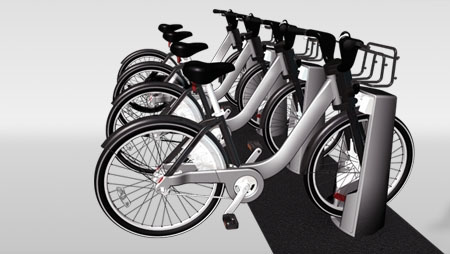
\includegraphics[scale=0.4]{dock}
\end{figure}

\textit{Requires a new system for docking a bicycle.}\\
\textit{Easily understood by the user.}\\
\textit{It integrates well with a locking mechanism.}

\bigskip
\btVFill
\tiny source of image: http://www.tuvie.com/wp-content/uploads/public-bike-system1.jpg
\end{frame}
\begin{comment}

\begin{frame}
\frametitle{Unlocking of Bicycles - On time}
\begin{figure}
\centering
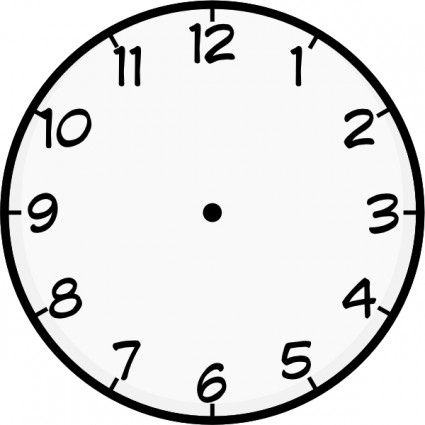
\includegraphics[scale=0.2]{clock}
\end{figure}

\textit{Easily understood by the user - just be there on time.}\\
\textit{Not at all flexible, hence not that user friendly.}

\bigskip
\btVFill
\tiny source of image: http://images.all-free-download.com/images/graphiclarge/purzen\_clock\_face\_clip\_art\_24896.jpg
\end{frame}

\begin{frame}
\frametitle{Unlocking of Bicycles - GPS}
\begin{figure}
\centering

\includegraphics[scale=0.1]{gps}
\end{figure}

\textit{Requires the user to carry a GPS device (not necessarily all users have such device).}\\
\textit{Can cause false unlocking.}

\bigskip
\btVFill
\tiny source of image: https://cdn3.iconfinder.com/data/icons/wireless/512/16-512.png
\end{frame}

\begin{frame}
\frametitle{Unlocking of Bicycles - QR Code}
\begin{figure}
\centering

\includegraphics[scale=0.1]{QR}
\end{figure}

\textit{Requires the user to have a device (often a smartphone) to take a picture of a QR code.}\\
\textit{May not be easily understood by all users.}\\

\bigskip
\btVFill
\tiny source of image: http://www.qrstuff.com/images/sample.png
\end{frame}

\begin{frame}
\frametitle{Unlocking of Bicycles - SMS}
\begin{figure}
\centering

\includegraphics[scale=0.1]{SMS}
\end{figure}

\textit{Requires a cellphone.}\\
\textit{Easy to use by most users.}\\
\textit{May be expensive for users without Danish subscription.}

\bigskip
\btVFill
\tiny source of image: http://www.fusionindia365.com/images/templatemo\_logo.png
\end{frame}
\end{comment}
\begin{frame}
\frametitle{Unlocking of Bicycles - Password}
\begin{figure}
\centering
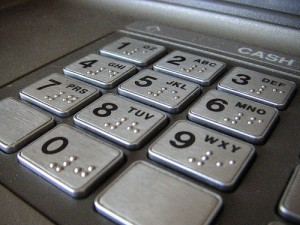
\includegraphics[scale=0.3]{password}
\end{figure}

\textit{Requires hardware for entering the password.}\\
\textit{Easily understood by the user.}\\
\textit{No requirements for the user.}

\bigskip
\btVFill
\tiny source of image: http://i.bnet.com/blogs/272104\_b9383b0487-300x225.jpg
\end{frame}

\begin{comment}

\begin{frame}
\frametitle{Booking Software - Mobile App}
\begin{figure}
\centering

\includegraphics[scale=0.1]{smartphone}
\end{figure}

\textit{Requires a smartphone with internet connection.}\\
\textit{Not accessible by everyone.}

\bigskip
\btVFill
\tiny source of image: http://cdns2.freepik.com/free-photo/smartphone\_318-23380.jpg
\end{frame}
\end{comment}



\begin{frame}
\frametitle{Booking Software - Website}
\begin{figure}
\centering

\includegraphics[scale=0.1]{web}
\end{figure}

\textit{Requires a browser.}\\
\textit{Can be accessed by everyone (e.g. go to the library)}\\
\textit{Can be adapted for mobile screen resolutions and take advantage of e.g. touch screen gestures.}

\bigskip
\btVFill
\tiny source of image: http://www.eventmanagerblog.com/uploads/2014/03/creating-perfect-event-websites.png
\end{frame}


\begin{frame}
\frametitle{Tracking of Bicycles - GPS}
\begin{figure}
\centering

\includegraphics[scale=0.15]{gps-signal}
\end{figure}

\textit{Requires a GPS device attached to each bicycle.}

\bigskip
\btVFill
\tiny source of image: http://cdns2.freepik.com/free-photo/receiving-gps-signal\_318-10003.jpg
\end{frame}
	\section{Internet of Things}

\begin{frame}
\frametitle{What is the Internet of Things?}
\begin{itemize}
\item Definition
\item Identification
\item Communication
\item Software
\end{itemize}
\end{frame}

\begin{frame}
\frametitle{Examples}
\begin{itemize}
\item Smart house
\item Intelligent energy management
\end{itemize}
\end{frame}

\begin{frame}
\frametitle{Relevance to our project}
\begin{itemize}
\item General idea grounded in the Internet of Things
\item Multiple things interconnected and available to users
\item Important aspects: Status, location, providing user control over system
\end{itemize}
\end{frame}

\section{Technologies}
\begin{frame}
\frametitle{Model-View-Controller}
\begin{itemize}
\item What is Model-View-Controller and how do we use it
\item Benefits: Clear code, organisation and architecture
\end{itemize}
\end{frame}

\begin{frame}
\frametitle{AJAX}
\begin{itemize}
\item Asynchronous updating, what is it and why should you use it?
\item Example: IMDb, giving a rating is asynchronous
\item How do we use it?
\end{itemize}
\end{frame}

\begin{frame}
\frametitle{SOAP}
\begin{itemize}
\item Simple Object Access Protocol, what is it?
\item Why SOAP over other methods? Standard protocol, easy to use and sufficient
\end{itemize}
\end{frame}
	\section{Implementation Details}
\begin{frame}
	\begin{center}
		\Huge Implementation Details
	\end{center}
\end{frame}
\begin{frame}
\frametitle{Overview}
\begin{itemize}
\item Database
\item Architecture
\item Synchronisation
\end{itemize}
\end{frame}

\begin{frame}
\frametitle{Database}
\begin{itemize}
	\item MySQL
	\item ER-Diagram $\rightarrow$ MySql Schema
\end{itemize}
	\begin{figure}
		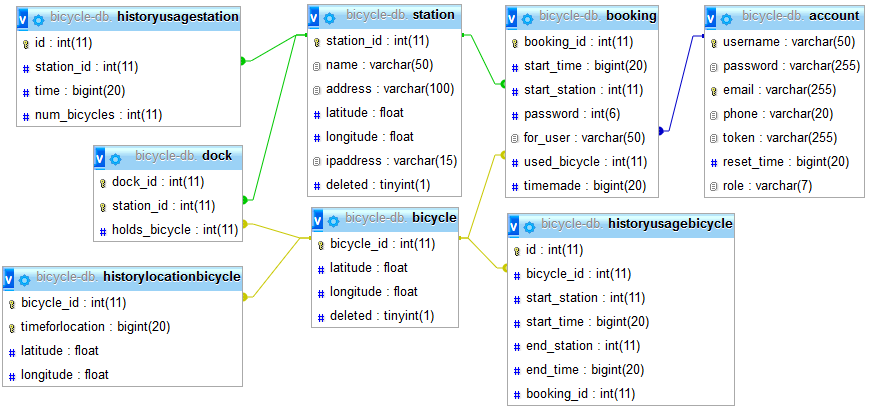
\includegraphics[scale=0.4]{DBtables}
	\end{figure}
\end{frame}


\begin{frame}
	\frametitle{Overall Architecture and Interaction}
		\begin{figure}
		\centering
			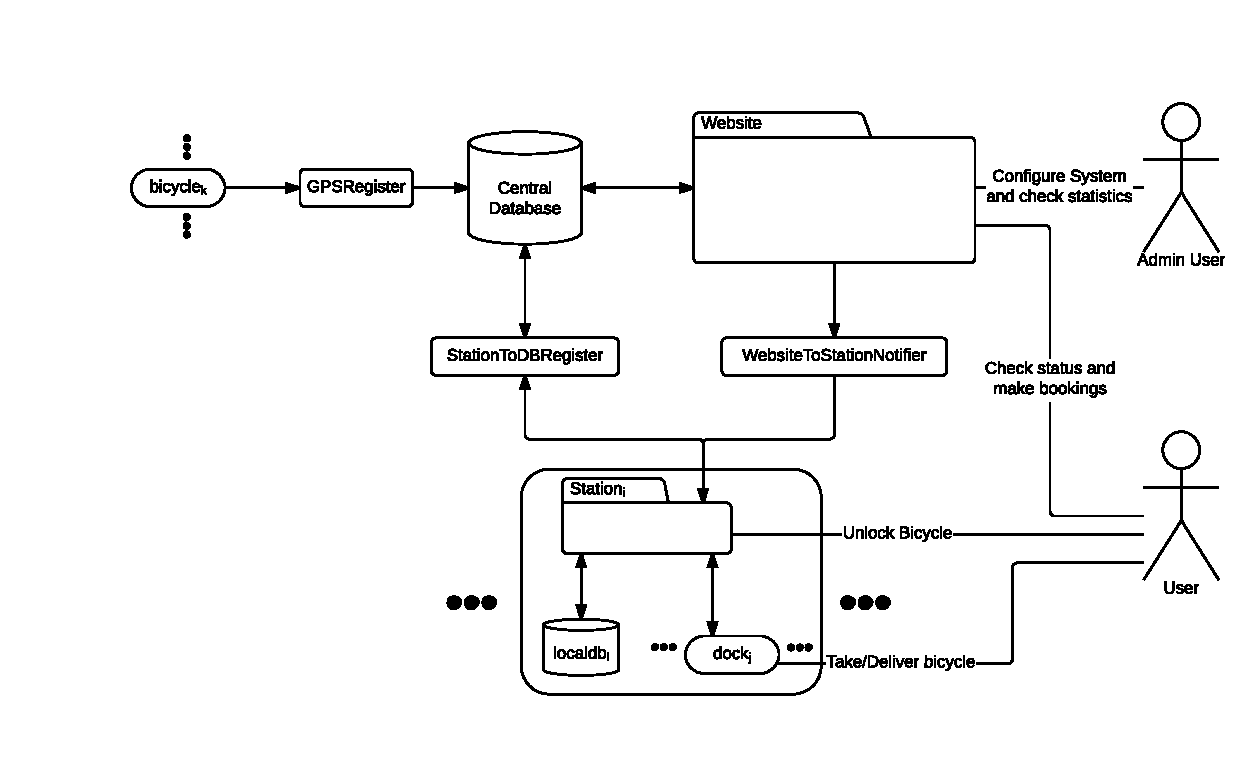
\includegraphics[scale=0.46]{architecture}
		\end{figure}
\end{frame}

\begin{frame}
	\frametitle{Overall Architecture and Interaction}
	\begin{figure}
		\centering
		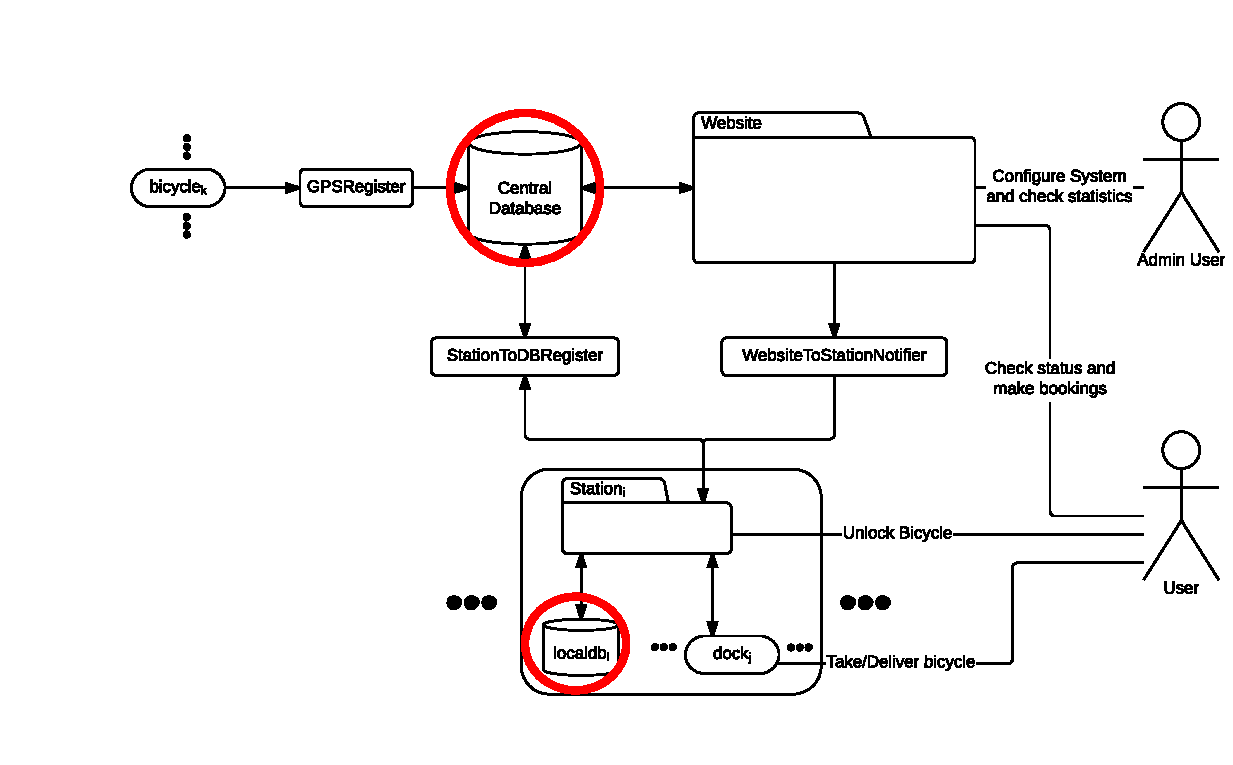
\includegraphics[scale=0.46]{arch1}
	\end{figure}
\end{frame}
\begin{frame}
	\frametitle{Overall Architecture and Interaction}
	\begin{figure}
		\centering
		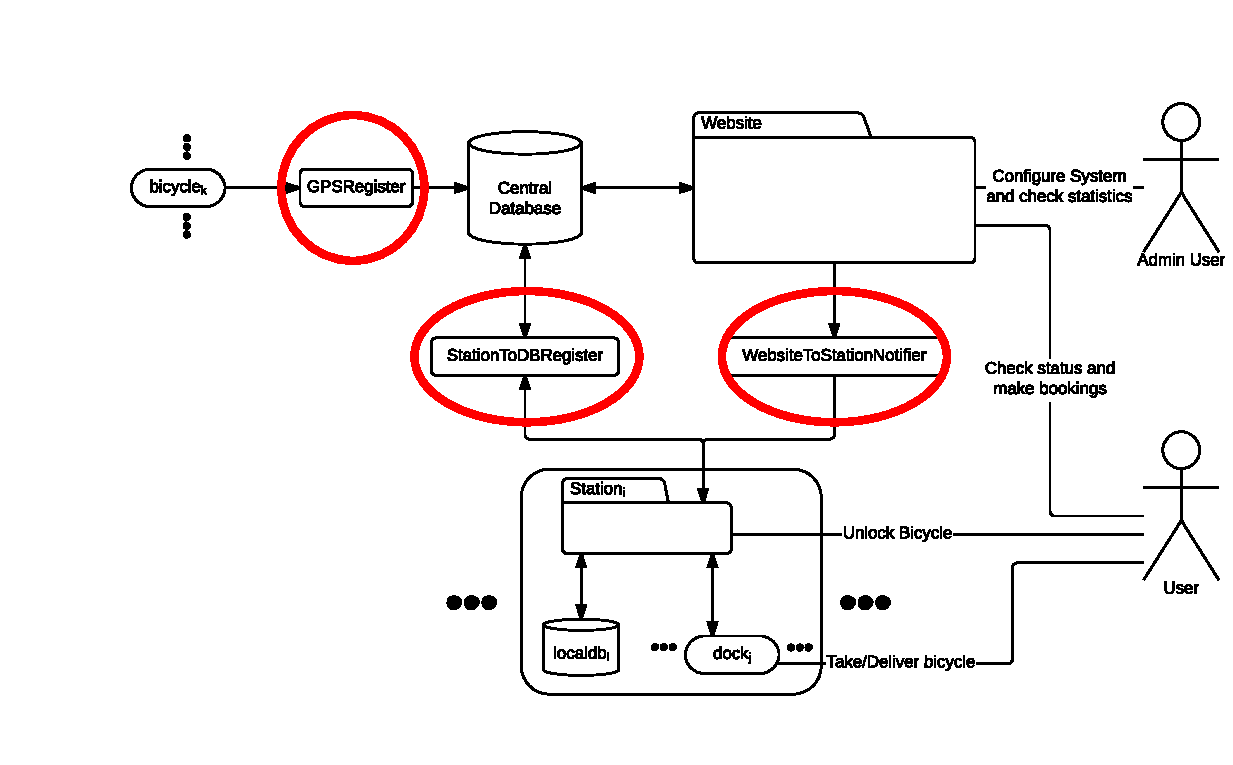
\includegraphics[scale=0.46]{arch2}
	\end{figure}
\end{frame}
\begin{frame}
	\frametitle{Overall Architecture and Interaction}
	\begin{figure}
		\centering
		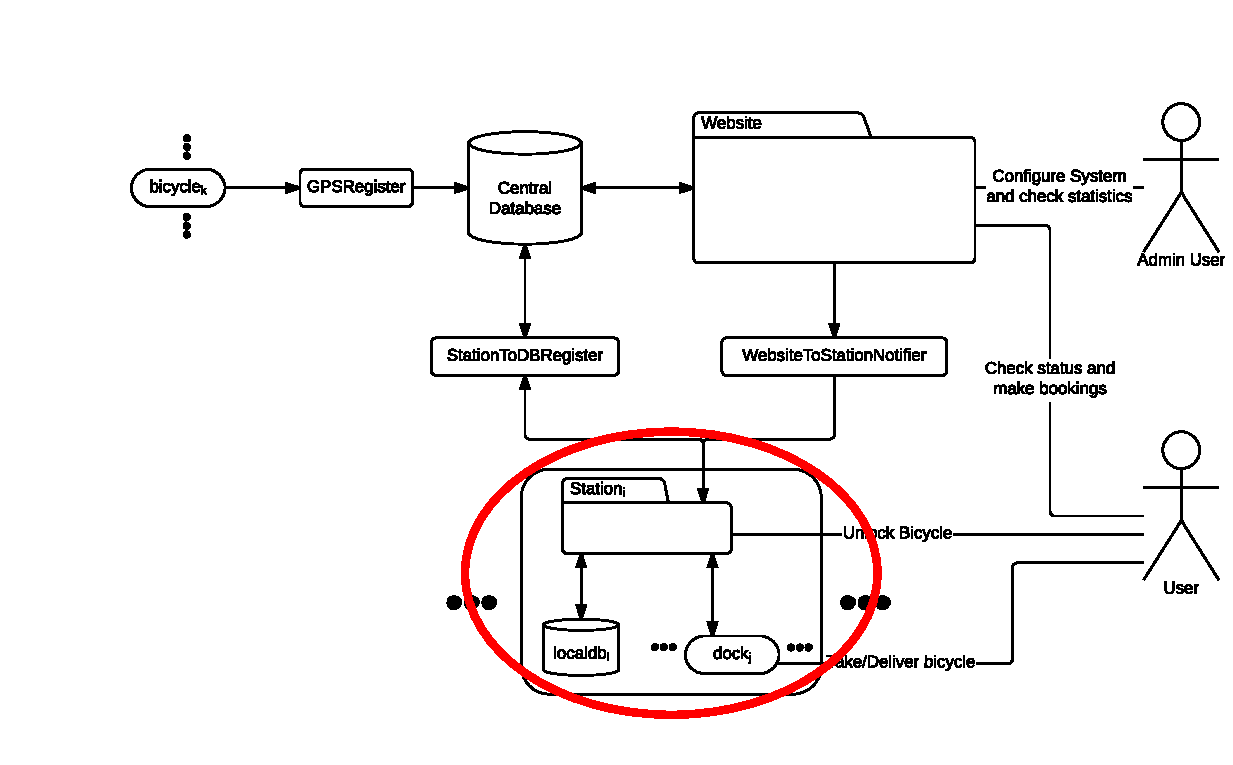
\includegraphics[scale=0.46]{arch3}
	\end{figure}
\end{frame}

\begin{frame}
	\frametitle{Overall Architecture and Interaction}
	\begin{figure}
		\centering
		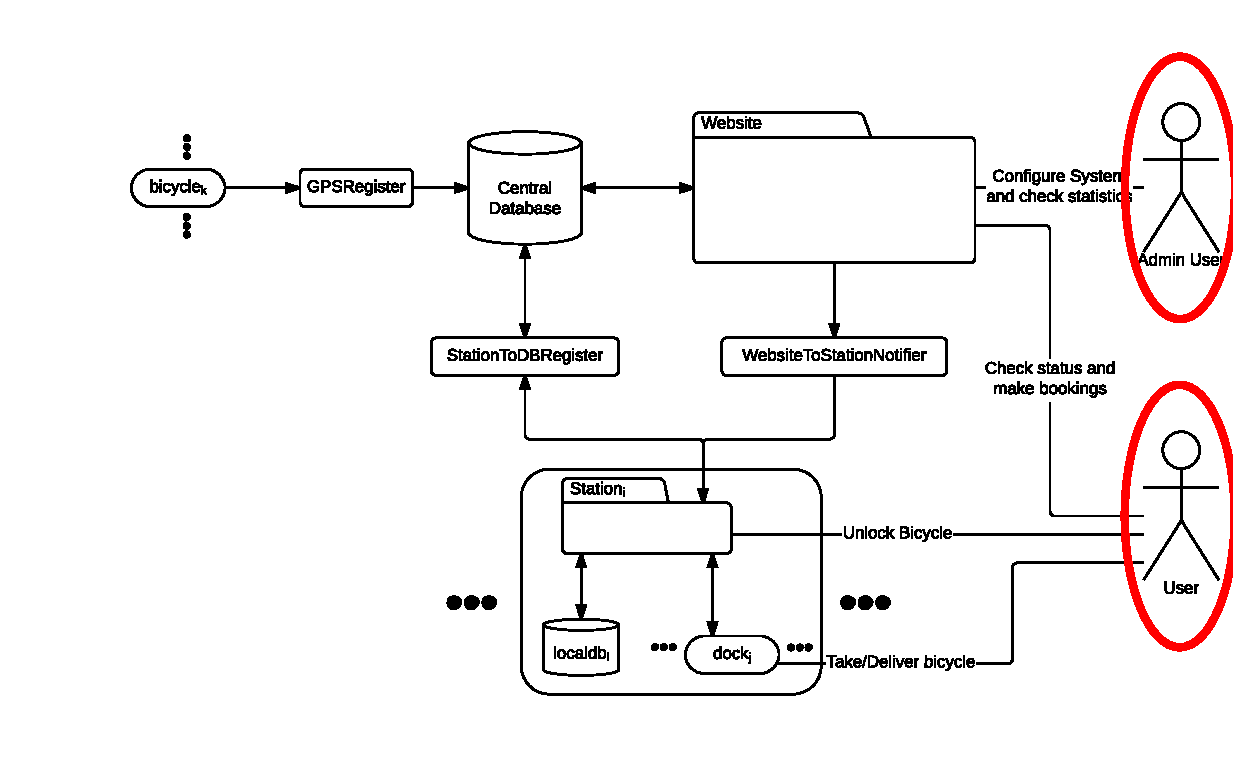
\includegraphics[scale=0.46]{arch4}
	\end{figure}
\end{frame}

\begin{frame}
	\frametitle{Webpage Architecture}
	\begin{figure}
	\centering
		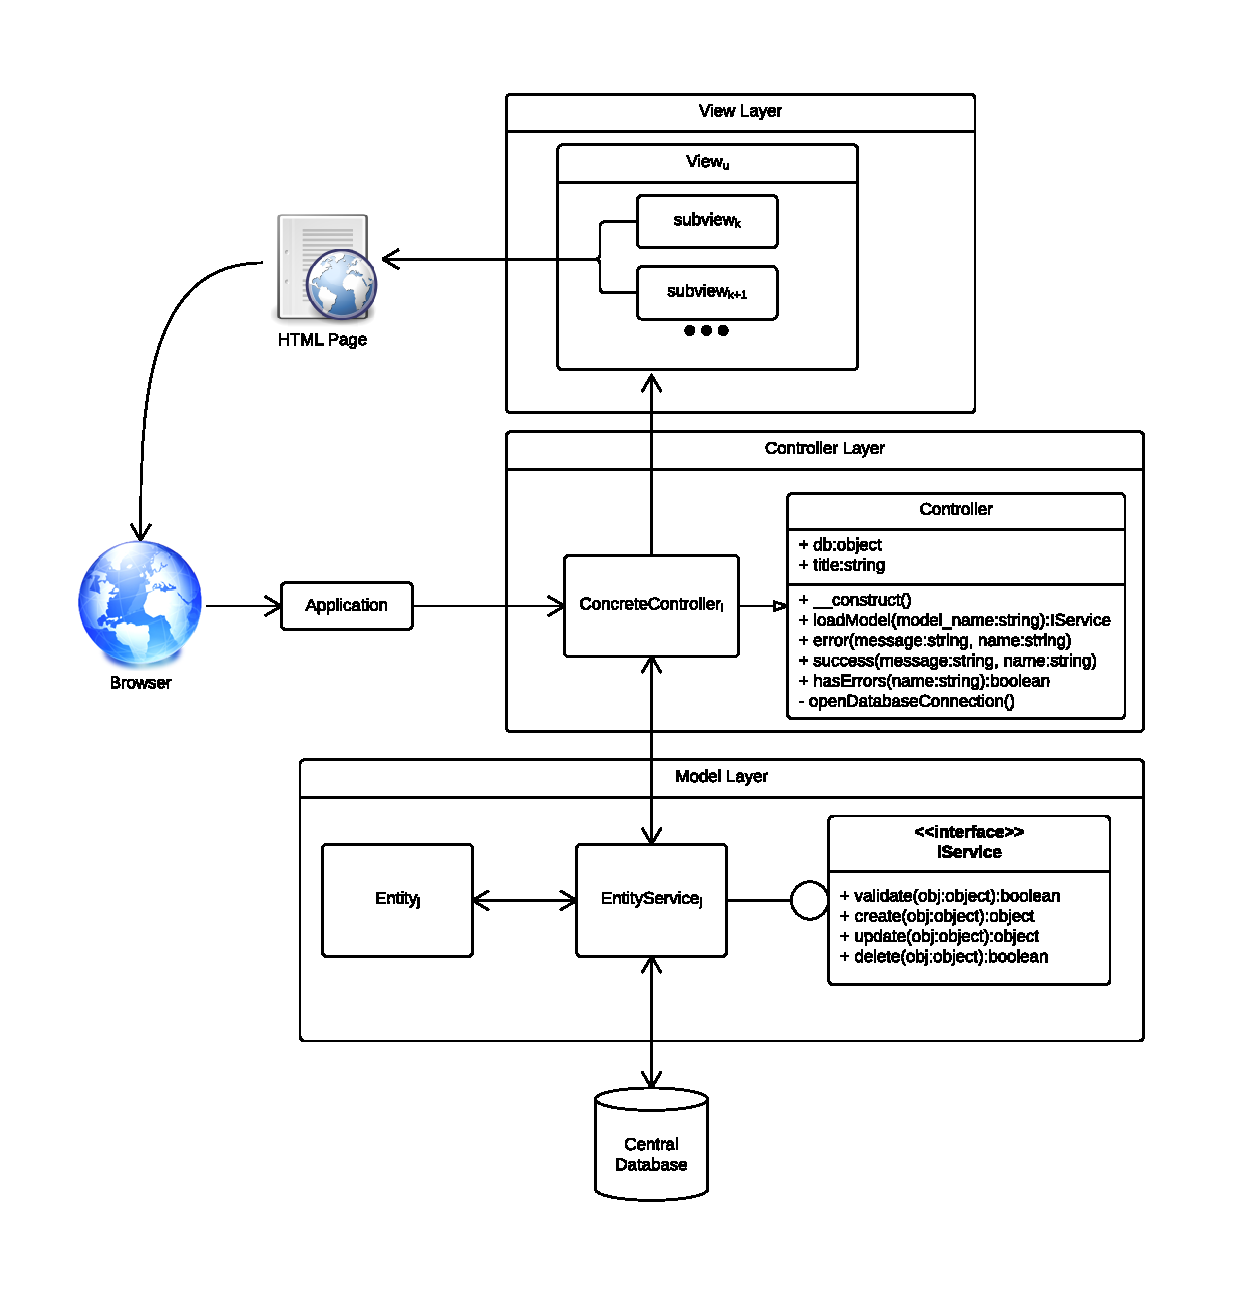
\includegraphics[scale=0.37]{ConcreteMVC}
	\end{figure}
\end{frame}


\begin{frame}
	\frametitle{Webpage Architecture}
	\begin{figure}
		\centering
		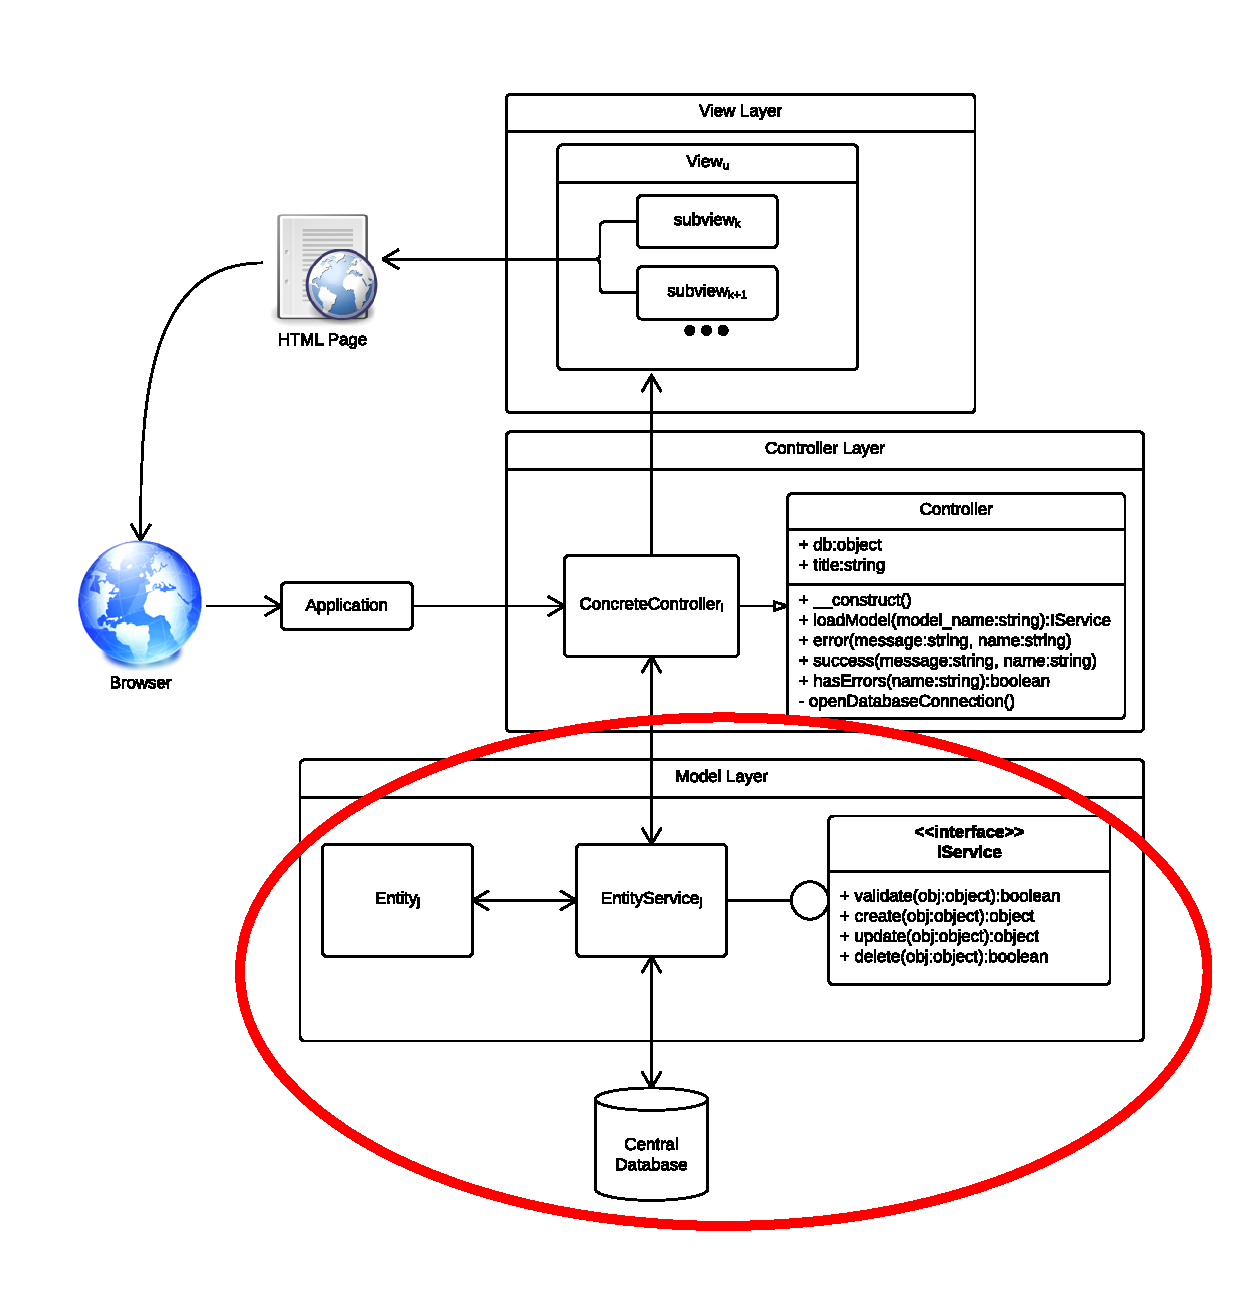
\includegraphics[scale=0.37]{mvc1}
	\end{figure}
\end{frame}


\begin{frame}
	\frametitle{Webpage Architecture}
	\begin{figure}
		\centering
		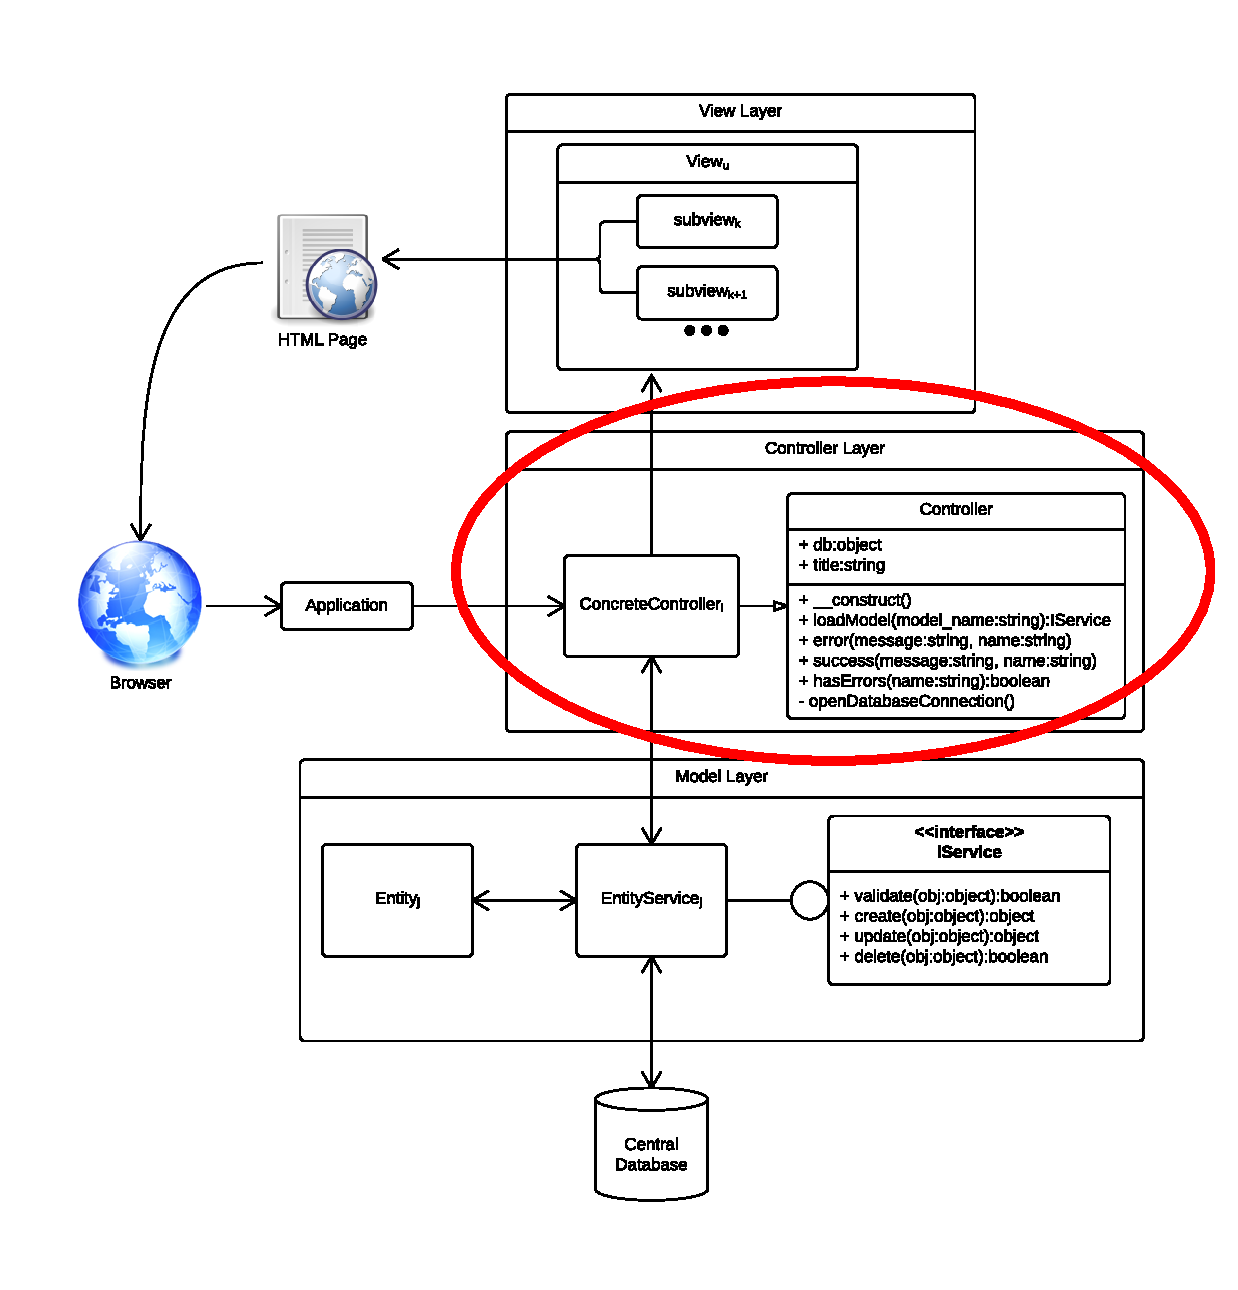
\includegraphics[scale=0.37]{mvc2}
	\end{figure}
\end{frame}


\begin{frame}
	\frametitle{Webpage Architecture}
	\begin{figure}
		\centering
		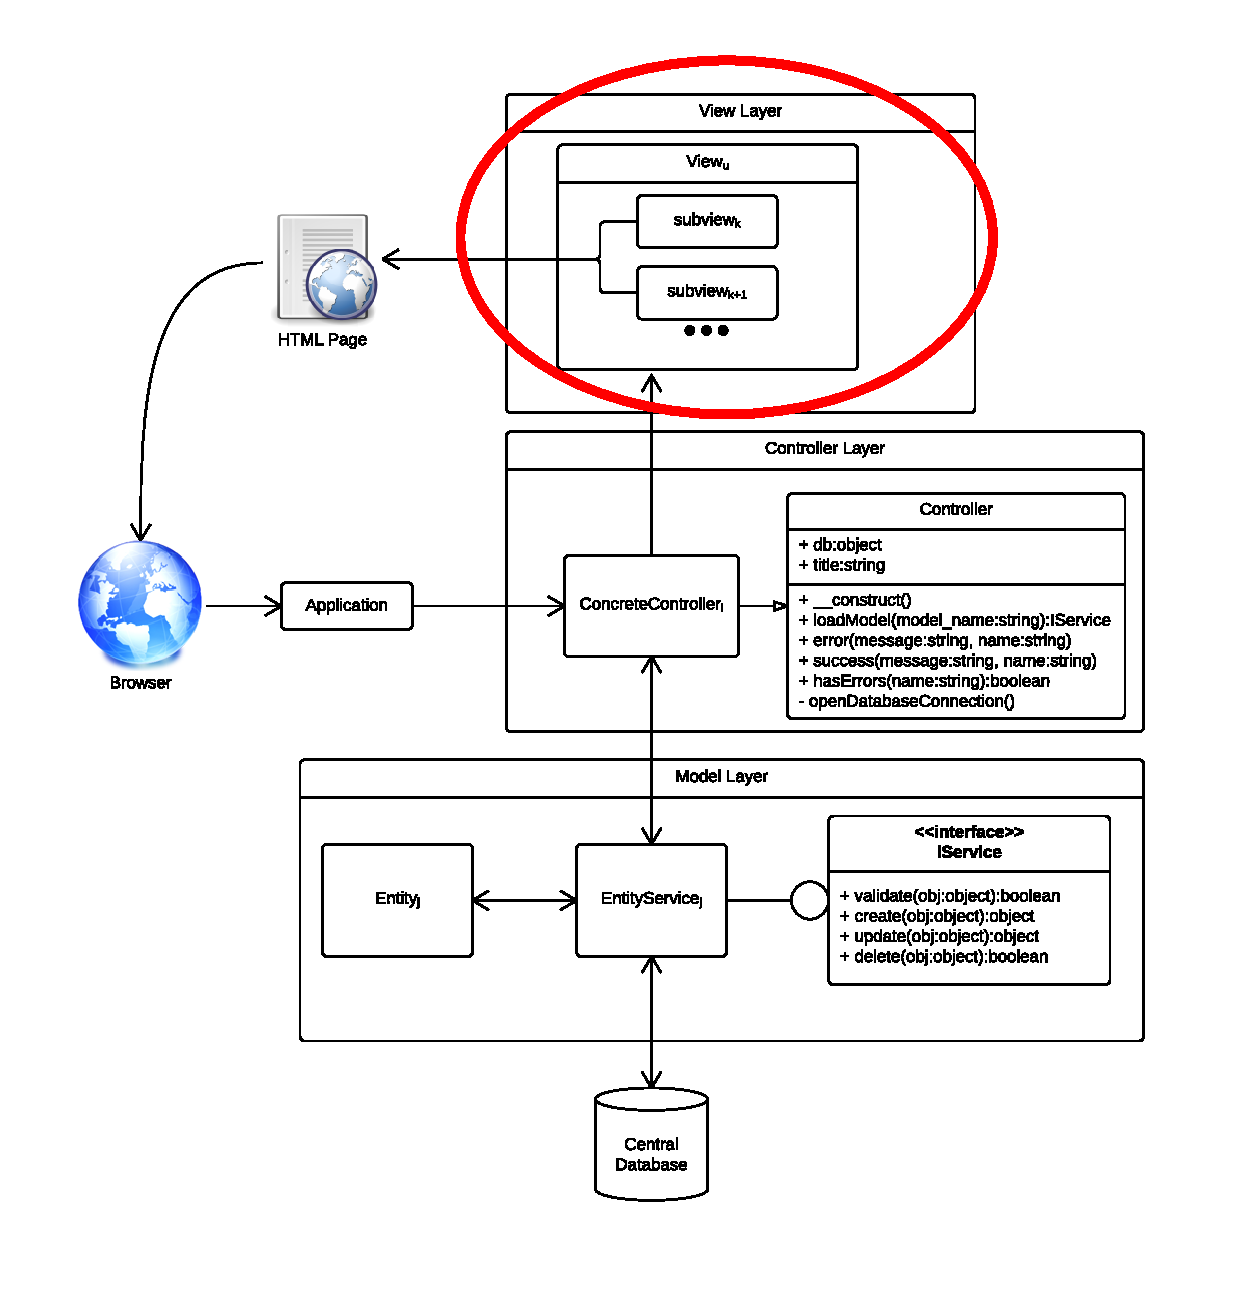
\includegraphics[scale=0.37]{mvc3}
	\end{figure}
\end{frame}


\begin{frame}
	\frametitle{Webpage Architecture}
	\begin{figure}
		\centering
		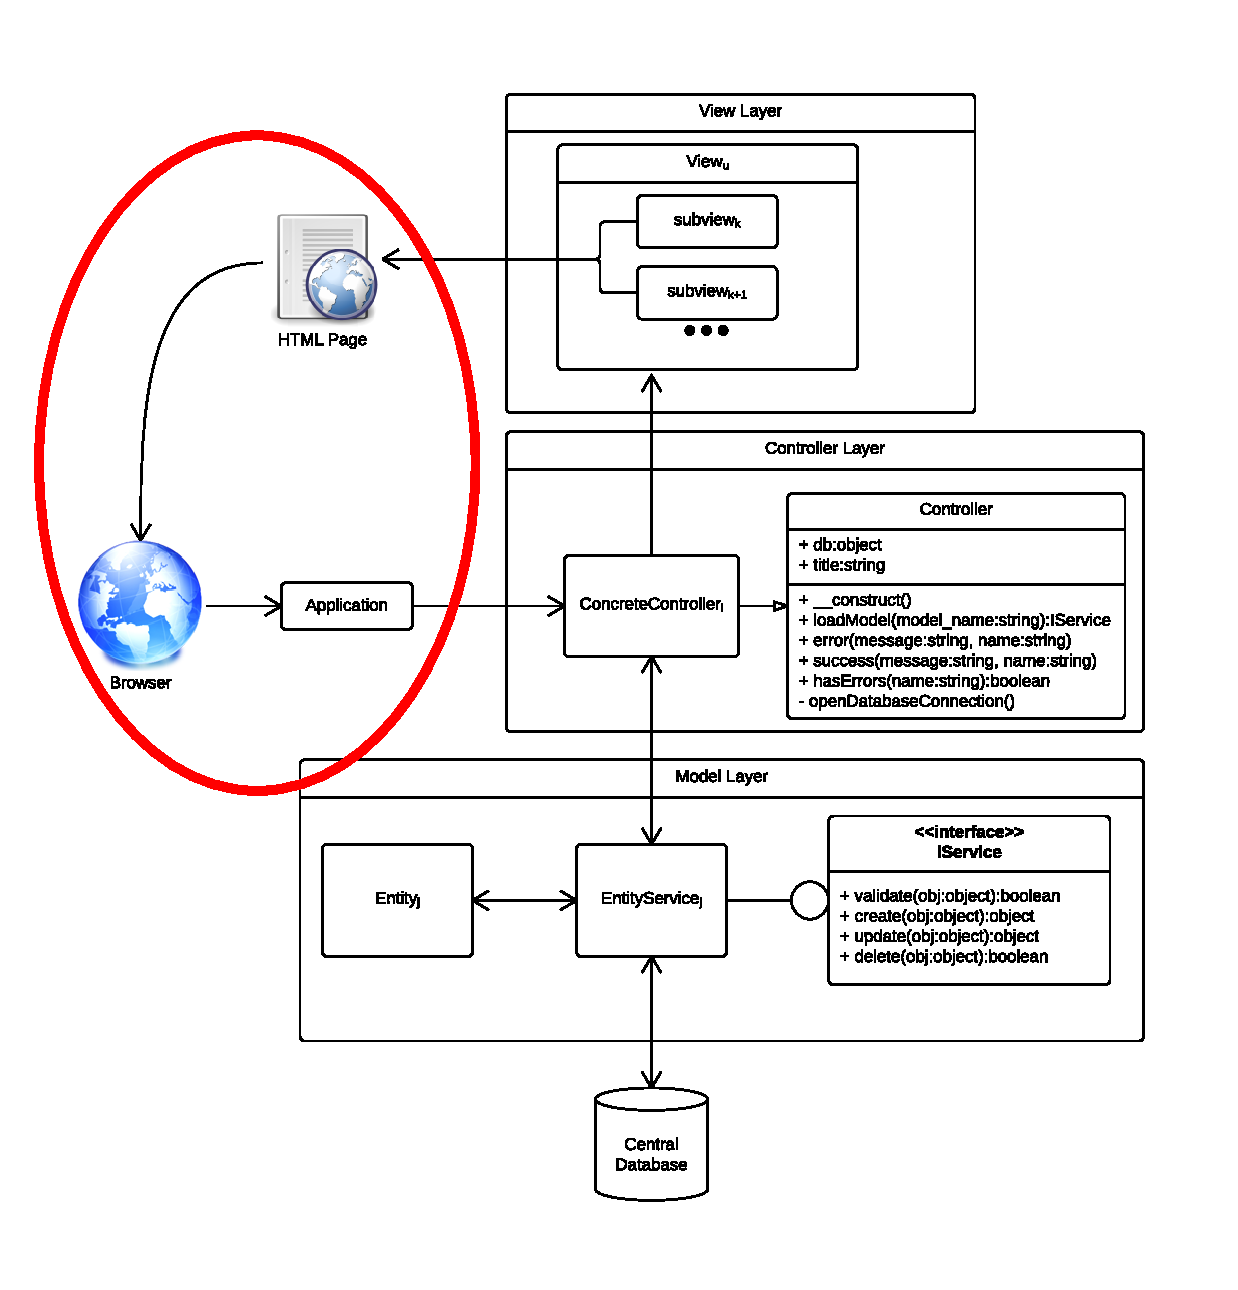
\includegraphics[scale=0.37]{mvc4}
	\end{figure}
\end{frame}

\begin{frame}
	\frametitle{Synchronisation}
	Watch out for:
	\begin{itemize}
		\item Inconsistent state
		\item Connection failures
	\end{itemize}
	\pause
	Issues:
	\begin{itemize}
		\item Bicycle locking/unlocking
		\item Removal/Insertion of bicycles
		\item Booking/Unbooking
	\end{itemize}
\end{frame}
	\section{Demonstration}
\begin{frame}
	\begin{center}
		\Huge Demonstration
	\end{center}
\end{frame}

\begin{frame}
\frametitle{Program Introduction}
\begin{itemize}
\item Website
\item Station Software
\item Simulated Hardware
\begin{itemize}
\item Stations and docks
\item Bicycles
\end{itemize}
\end{itemize}
\end{frame}

\begin{frame}
	\begin{center}
		\Huge Demonstration
	\end{center}
\end{frame}
	\section{Test}
\begin{frame}
\begin{center}
\Huge Test
\end{center}
\end{frame}

\begin{frame}
\frametitle{Overview}
\begin{itemize}
	\item Testing
	\item Discussion
	\item Conclusion
\end{itemize}	
\end{frame}

\begin{frame}
\frametitle{Unit Testing}
\begin{itemize}
	\item Binding Parameters MySQLi
	\item Incorrect Method Calls
	\item Type Checking
\end{itemize}
\end{frame}

\begin{frame}
\frametitle{Usability Test}
\begin{itemize}
	\item Field Reset
	\item Error Messages
	\item Finding History
	\item Confirmation Box
\end{itemize}
\end{frame}

\section{Discussion \& Conclusion}
\begin{frame}
\begin{center}
\Huge Discussion \& Conclusion
\end{center}
\end{frame}
\begin{frame}
\frametitle{Decisions}
\begin{itemize}
	\item Static Booking
	\item Designed for PC
	\item Hardware vs. Simulation
\end{itemize}
\begin{figure}
	\centering
	\includegraphics[scale=0.15]{Media/Web}
\end{figure}
\end{frame}

\begin{frame}
\frametitle{Further Development}
\begin{itemize}
	\item Mobile Application
	\item Usability Test
	\item Hotspot Detection
\end{itemize}
\begin{figure}
\centering
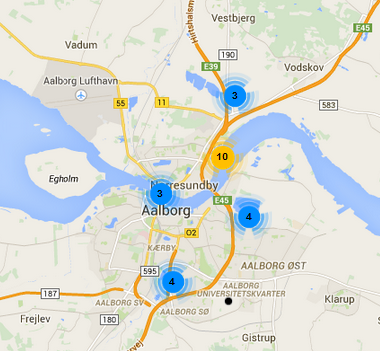
\includegraphics[scale=0.5]{MarkerClusterer}
\end{figure}
\end{frame}

\begin{frame}
\frametitle{Conclusion}
\begin{center}
	\textit{What are the requirements for a city bicycle booking and positioning system?}
\end{center}

\begin{itemize}
	\item[\color{green}\checkmark] Provide status of bicycles
	\item[\color{green}\checkmark] Give an option to book a bicycle
	\item[\color{green}\checkmark] Track bicycles
	\item[\color{green}\checkmark] Collect data for analysis
	\item[\color{red}$\div$] Predict usage of bicycles
\end{itemize}
\end{frame}

\begin{frame}
	\frametitle{Conclusion}
	\begin{center}
		\textit{How can the booking and positioning system be designed and implemented, within the context of the Internet of Things?}
	\end{center}

\begin{itemize}
	\item[\color{green}\checkmark] Bicycles
	\item[\color{green}\checkmark] Stations
	\item[\color{green}\checkmark] Database
\end{itemize}
\end{frame}

\begin{frame}
	\frametitle{Conclusion}
	\begin{center}
		\textit{Why should the developed system be used over the currently used system?}
	\end{center}
	
	\begin{itemize}
		\item[\color{green}\checkmark] Extra Features
		\item[\color{orange}---] Static System
		\item[\color{green}\checkmark] Pick and Choose Functionality
	\end{itemize}
\end{frame}

\begin{frame}
	\frametitle{Conclusion}
	\begin{center}
		\textbf{It is possible to develop a system for Aalborg Bycykel that is user friendly and manageable, within the context of the Internet of Things}
	\end{center}
\end{frame}
	\bgroup
	\setbeamercolor{background canvas}{bg=black}
	\begin{frame}[plain]{}
	\addtocounter{framenumber}{-1}	
		\begin{center}
		%\textcolor{white}{END}
		\end{center}
	\end{frame}
	\egroup
	
\end{document}
